\documentclass[xcolor={x11names}]{beamer}
\usetheme{Frankfurt}

\usepackage{unicode-math}
\usepackage{amsmath}
\usepackage{graphicx}
\usepackage{amssymb}
\usepackage{remreset}
\usepackage{mathtools}
\usepackage{latexsym}
\usepackage{cancel}
\usepackage{hyperref}
\usepackage{xspace}
\usepackage{textcomp}
\setmonofont{FreeMono}

\usepackage[style=authoryear]{biblatex}
\hypersetup{colorlinks=true,urlcolor=DodgerBlue4,linkcolor=Firebrick4,citecolor=Firebrick4}

% link over the authors as well.
\DeclareCiteCommand{\cite}
{\usebibmacro{prenote}}
{\usebibmacro{citeindex}%
  \printtext[bibhyperref]{\usebibmacro{cite}}}
{\multicitedelim}
{\usebibmacro{postnote}}

% tiny circles without subsections
\makeatletter
\@removefromreset{subsection}{section}
\makeatother
\setcounter{subsection}{1}

\bibliography{refs}


\title{Generalized Veltman Semantics in Agda}
\subtitle{Master's thesis \\ {\scriptsize Master in Pure and Applied Logic}}
\author[Mas]{Jan Mas Rovira\inst{1} \\[1ex] {\footnotesize Supervisors:  Joost J.
    Joosten\inst{1} \and Luka Mikec\inst{2}}}
\institute[UB, UZ]{\inst{1} Universitat de Barcelona \and
  \inst{2} University of Zagreb}
\date[Nov 2020]{November 27th 2020}
\titlegraphic{ 
\includegraphics[width=4cm]{img/ub-logo.pdf}}

\newcommand{\prin}[1]{\ensuremath{\textbf{\textup{#1}}}\xspace}
\newcommand{\il}{\prin{IL}}
\newcommand{\ilm}{\prin{ILM}}
\newcommand{\gl}{\prin{GL}}
\newcommand{\zf}{\prin{ZF}}
\newcommand{\ch}{\prin{CH}}
\newcommand{\veql}{\prin{(V=L)}}
\newcommand{\rn}{\ensuremath{\prin{R}^n}\xspace}
\newcommand{\rsn}{\ensuremath{\prin{R}_n}\xspace}
\newcommand{\principle}[1]{\text{$\mathsf{#1}$}}

\begin{document}

\frame{\titlepage}

\section{Introduction}
\begin{frame}
  \frametitle{Introduction}
  \begin{itemize}
  \item Agda is a \textbf{proof assistant} based on dependent type theory.
    \break \pause
  \item Generalized Veltman semantics are a kind of relational semantics (à la
    Kripke) for \textbf{interpretability logics}.
  \end{itemize}
\end{frame}

\begin{frame}
  \frametitle{Examples of interpretations}
  Examples of interpretations (\cite{visser1997overview}):
  \pause
  \vspace{0.4cm}
  \begin{itemize}
  \item The interpretation of arithmetic in set theory.
    \pause
  \item Gödel's interpretation of $\zf+\veql$ in \zf
       shows consistency of \zf + \ch w.r.t. \zf.
    \pause
  \item The interpretation of elementary syntax in arithmetic. Important for
    Gödel's incompleteness theorems.
  \end{itemize}
\end{frame}

\section{Interpretability Logics}
\begin{frame}
  \frametitle{Interpretability Logics}
  In the logic of provability \gl we have that:
  \begin{itemize}
    \item $□A$ means ``A is provable''.
    \item $♢A$ means ``A is consistent''. Note that $♢A=¬□¬A$.
  \end{itemize}
  The aim of \gl is to describe and prove the structural behaviour of the
  provability predicate.

  \pause \vspace{0.2cm}

  Interpretability logics extend the provability logic \gl. The language is
  $⟨→,⊥,□,▷⟩$ and we can define $♢,∧,∨$ in the usual way.
  \begin{itemize}
  \item $A▷B$ means ``T + A* interprets T + B*''.
  \end{itemize}
  Given a reasonable arithmetical theory $\prin{T}$ the aim is to find the logic
  $\prin{IL(T)}$ which describes the structural behaviour of its
  interpretability predicate.
  \[\prin{IL(T)}⊢A⇔ \prin{T}⊢A^*\text{, for any realisation *.} \]

\end{frame}

\begin{frame}
  \frametitle{Arithmetical realisation}
  Given an arithmetical theory $\prin{T}$ with language $ℒ$, an arithmetical
  realisation $*$ is a map from interpretability formulas to sentences of
  $ℒ$.
  \begin{itemize}
    \item $p^*$ is a sentence of $ℒ$;
    \item $⊥^*$ is $0=1$;
    \item $(A \to B)^* = A^* \to B^*$;
    \item $(A \rhd B)^* = \mathsf{Int}_{\prin{T}}(\ulcorner A^* \urcorner, \ulcorner B^*\urcorner)$;
    \item $(□A)^* = \mathsf{Prov}_{\prin{T}}(\ulcorner A^* \urcorner)$.
  \end{itemize}
  %   \pause
  %   We are concerned with interpretability with respect to some theory $T$.
  %   \[T+A▷T+B\]
\end{frame}

\begin{frame}
  \frametitle{Logic \il}
  The logic \il is contained in almost all interpretability logics.

  \vspace{0.3cm} The rules are modus ponens and necessitation. It has all the
  theorems of \gl plus the following axioms schemes: \pause

  % In particular, you should add a pair of brackets in J3 and two in J2, on in
  % J4 (we’re not type-theorists)
  \begin{itemize}
  \item J1: $□ (A → B) → (A ▷ B)$;
    \pause
  \item J2: $(A ▷ B) ∧ (B ▷ C) → (A ▷ C)$;
    \pause
  \item J3: $(A ▷ C) ∧ (B ▷ C) → (A ∨ B) ▷ C$;
    \pause
  \item J4: $(A ▷ B) → (♢ A → ♢ B)$;
    \pause
  \item J5: $♢ A ▷ A$.
  \end{itemize}
\end{frame}

\begin{frame}
  \frametitle{Logic \ilm}

  The logic ILM is defined as \il + \prin{M}, where
  \[\prin{M}≔ A ▷ B → (A ∧ □ C) ▷ (B ∧ □ C).\]

  The theorems of $\textsf{ILM}$ are the set of interpretability principles that
  are always provable in theories which are $Σ_1$ sound and have full induction.
  An example of such theory is $\textsf{PA}$, thus $\prin{IL(PA)}=\ilm$
  (\cite{berarducci1990interpretability,shavrukov1988logic}).

  % TODO MISSING REFERENCE

\end{frame}

\section{Semantics and frame conditions}
\begin{frame}
  \frametitle{Generalized Veltman Semantics (Verbrugge 1992)}
  A \textbf{generalized Veltman frame} (GVF) is a tuple $⟨W,R,\{S_w:w∈W\}⟩$ with
  $R⊆W×W$ and $S_w⊆W×(𝒫(W)∖\{∅\})$.\\ We write $uS_wY$ instead of $⟨u,Y⟩∈S_w$.
  \begin{itemize}
    \item $R$ is transitive and conversely well-founded;
    \item if $uS_wY$ then $wRu$ and $\{v:wRv\}⊆Y$;
    \item if $wRu$ then $uS_w\{u\}$;
    \item if $wRuRv$ then $uS_w\{v\}$;
    \item if $uS_wY$ and for all $y∈Y$ we have $yS_wZ_y$ then $uS_w\left(⋃_{y∈Y}Z_y\right)$.
  \end{itemize}

  \pause
  \vspace{0.3cm}
  A \textbf{generalized Veltman model} (GVM) is a tuple $⟨W,R,S,V⟩$ where
  $⟨W,R,S⟩$ is a GVF and $V⊆W×Var$ is a valuation.

  \vspace{0.2cm}
  Soundness and completeness w.r.t to \il.
\end{frame}

\begin{frame}
  \frametitle{Generalized Veltman Semantics}
  Given a GVM $⟨W,R,S,V⟩$ we define $⊩\ ⊆W×Fm$ as follows:
  \begin{itemize}
    \item $w⊮⊥$;
    \item $w⊩p$ iff $⟨w,p⟩∈V$;
    \item $w⊩A→B$ iff $w⊩A$ implies $w⊩B$;
    \item $w⊩□A$ iff for all $u$ such that $wRu$ we have $u⊩A$;
    % \item $w⊩♢A$ iff there is some $u$ such that $wRu$ and $u⊩A$;
      \pause
    \item $w⊩A▷B$ iff $wRu$ and $u⊩A$ implies that there exists some $Y$ such
      that $uS_wY$ and for all $y∈Y$ we have $y⊩B$.
  \end{itemize}
  \begin{figure}[t]
    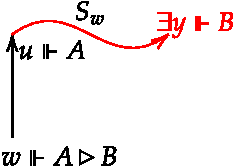
\includegraphics[scale=0.8]{img/ArhdB-ord}
    \centering
  \end{figure}
\end{frame}

\begin{frame}
  \frametitle{Frame conditions}
  Given any principle $P$ we say that a first order (or higher order) formula
  $(P)_{gen}$ is the \textbf{frame condition} for $P$ if for any GVF $F$ we have
  \[F⊨(P)_{gen}⇔F⊩P,\]
  where $F⊩P$ iff $⟨F,V⟩⊩P$ for any valuation $V$.
  \pause

  \vspace{0.7cm}

  Example: The frame condition $(M)_{gen}$ is
  \[ ∀w,x,V(xS_wV⇒ ∃V'⊆V(xS_wV',∀v'∈V'∀z(v'Rz⇒xRz))).\]
\end{frame}

\begin{frame}
  \frametitle{\prin{IL(All)} and the series of principles \rn and \rsn}
  The logic \prin{IL(All)} is the intersection of interpretability
  logics of all reasonable arithmetical theories.

  \pause

  The best known lower bound for \prin{IL(All)} is $\prin{ILWR}^n\prin{R}_n$.

  The series of principles \rn and \rsn are due to \cite{two-new-series}.

  \vspace{0.2cm}
  Definition of $\rn$:
  \begin{flalign*}
    U_0 &≔ ♢¬(D_0▷¬C) \\
    U_{r+1} &≔ ♢((Dᵣ▷D_{r+1}) ∧ Uᵣ) \\
    R⁰& ≔ A ▷ B → ¬ (A ▷ ¬ C) ▷ B ∧ □ C \\
    R^{n+1}& ≔ A ▷ B → ((D_{n}▷A) ∧ U_{n}) ▷ B ∧ □ C
  \end{flalign*}

  \pause
  We have found frame conditions for generalized Veltman semantics for $R^n$ and
  $R_1$. The proofs have been formalised in Agda.
\end{frame}

\section{Agda formalisation}
\begin{frame}[fragile]
  \frametitle{Agda}
  Agda is a \textbf{proof assistant} based on an extension of Martin Löf's constructive
  type theory.

  \vspace{0.3cm}
  \pause
  Papers that use Agda (\textasciitilde 200):

  \begin{itemize}
  \item \href{https://wiki.portal.chalmers.se/agda/Main/PapersUsingAgda}{wiki.portal.chalmers.se/agda/Main/PapersUsingAgda}

  \item \href{https://researchr.org/bibliography/agda-papers/publications}{researchr.org/bibliography/agda-papers/publications}
  \end{itemize}

  \pause

  \vspace{0.3cm}
  How we prove things in Agda?
  \begin{itemize}
  \item The \textcolor{blue}{type} expresses the \textcolor{blue}{property}.
  \item The \textcolor{red}{term} is a constructive \textcolor{red}{proof}.
  \end{itemize}

\end{frame}

\begin{frame}[fragile]
  \frametitle{Agda theorem example}
  Given any GVM $M=⟨W,R,S,V⟩$, world $w∈W$ and formulas $A,B$ we have that
  \[M,w⊩□ (A → B) → A ▷ B\]
  \pause
  The property as an Agda type:
\begin{verbatim}
  ∀ {W R S V}
    {M : Model W R S V}
    {w : W}
    {A B : Fm}
   →
    M , w ⊩ □ (A ↝ B) ↝ A ▷ B
\end{verbatim}
\end{frame}

\begin{frame}
  \frametitle{Agda formalisation}
  Our Agda library includes (\textasciitilde 5k lines of code):
  \begin{itemize}
  \item Definition of ordinary and generalized Veltman Semantics.
  \item Definition of logic IL and many of the relevant interpretability
    principles in conjunction with their proven frame conditions. These include
    $\principle{M}$, $\principle{P_0}$, $\principle{R}$, $\principle{M_0}$ for
    both semantics and $\principle{R^n}$, $\principle{R_1}$ for generalized
    semantics.
  \item A verified embedded domain specific language for Hilbert style proofs
    for the logic \il.
  \item And much more... (see reference \cite{MasRovira:2020:MastersThesis}).
  \end{itemize}
\end{frame}

\begin{frame}[fragile]
  \frametitle{Hilbert style proofs in Agda}

  Let us show $⊢_{\il}A▷A$ using our language.
  \pause
  \vspace{0.6cm}
\begin{semiverbatim}
⊢A▷A : \{A : Fm\} → [] ⊢ A ▷ A
\uncover<3->{⊢A▷A \{A\} =
  begin[ 0 ] A ↝ A                 By ⊢A↝A}
\uncover<4->{       [ 1 ] □ (A ↝ A)             ByNec 0}
\uncover<5->{       [ 2 ] □ (A ↝ A) ↝ (A ▷ A)   By J1}
\uncover<6->{       [ 3 ] A ▷ A                 ByMP 2 , 1
       ■}
\end{semiverbatim}
\end{frame}

\begin{frame}
  \frametitle{Open source}
  \centering
  \href{https://gitlab.com/janmasrovira/interpretability-logics}{gitlab.com/janmasrovira/interpretability-logics}
\end{frame}

\begin{frame}
  \centering \Huge Thank you!
\end{frame}

\begin{frame}[allowframebreaks]
  \frametitle{References}
  \nocite{joosten2020overview}
  \nocite{Verbrugge}
  \printbibliography
\end{frame}

\end{document}